\documentclass[article,aoas,preprint]{imsart}

\usepackage[nofiglist, nomarkers]{endfloat}
\usepackage{algorithm}
\usepackage{graphicx}
\usepackage{amsmath}
\usepackage{amssymb}
\usepackage{amsfonts}
\usepackage{amsthm}
\usepackage{xfrac}
\usepackage{float}
\usepackage{fullpage}
\RequirePackage[colorlinks,citecolor=blue,urlcolor=blue]{hyperref}

% override imsart settings for final project
\startlocaldefs
\setattribute{title}{size} {\fontseries{bx}\fontsize{14}{16}\selectfont\mathversion{bold}\spaceskip.5em}
\setattribute{journal}{name}{PH240F: Statistical Genomics II}
\setattribute{author}{prefix}{}
\setattribute{volume}{title}{Spring 2014---Final Project}

\makeatletter
\let\@fnsymbol\@arabic
\makeatother
\numberwithin{equation}{section}
\theoremstyle{plain}
\newtheorem{thm}{Theorem}[section]
\newtheorem{lemma}{Lemma}[section]
\newtheorem{definition}{Definition}
\newtheorem{Rule}{Rule}
\newtheorem*{notation}{Notation}
\endlocaldefs

% my standard setup 
\newcommand{\der}[2]{\frac{d #1}{d #2}} % for derivatives
\newcommand{\V}[1]{\ensuremath{\mathbf{#1}}} % for vectors
\newcommand{\gv}[1]{\ensuremath{\mbox{\boldmath$ #1 $}}} % for vectors of Greek letters
\newcommand{\pd}[2]{\frac{\partial #1}{\partial #2}}  % for partial derivatives
\newcommand{\grad}[1]{\gv{\nabla} #1} % for gradient
\newcommand{\reals}{\mathbb{R}}
\newcommand{\ints}{\mathbb{Z}}
\newcommand{\blank}{\underline{\hspace*{1in}}}
\newcommand{\PMF}{\mathrm{PMF}}
\newcommand{\PDF}{\mathrm{PDF}}
\newcommand{\CDF}{\mathrm{CDF}}
\newcommand{\N}[2]{\mathcal{N}\left(#1,#2\right)}
\newcommand{\empavg}[2]{\frac{1}{#1}\sum_{i=1}^{#1}\left[#2\right]}
\newcommand{\E}[1]{{\rm I\kern-.3em E}\left[#1\right]}
\newcommand{\Var}[1]{\mathrm{Var}\left[#1\right]}
\newcommand{\Cov}[1]{\mathrm{Cov}\left[#1\right]}
\def\ci{\perp\!\!\!\perp}
\newcommand{\argmax}[1]{\underset{#1}{\operatorname{argmax}}}
\newcommand{\argmin}[1]{\underset{#1}{\operatorname{argmin}}}
\newcommand{\iid}{\stackrel{\mathrm{iid}}{\sim}}
\newcommand{\logit}[1]{\operatorname{logit}({#1})}
\providecommand{\e}[1]{\ensuremath{\times 10^{#1}}}
\newcommand{\Tr}[1]{\mathrm{Tr}\left(#1\right)}
\newcommand{\adim}[2]{\underset{\scriptscriptstyle #1}{#2\strut}}

\newcommand{\fix}[1] { \textcolor{red} {
{\fbox{ {\bf Fix:} \ensuremath{\blacktriangleright }} {\bf #1}
\fbox{\ensuremath{\blacktriangleleft} } } } }



\begin{document}

\begin{frontmatter}

\title{Classification for Renal Cell Carcinomas}
\runtitle{Renal cell carcinomas classification}

\begin{aug}
\author{\fnms{Alex} \snm{Anderson},\thanksref{t1}\ead[label=e1]{aga@berkeley.edu}}
\author{\fnms{K. Jarrod} \snm{Millman},\thanksref{t2}\ead[label=e2]{millman@berkeley.edu}}
\and
\author{\fnms{Lara} \snm{Troszak}\thanksref{t2}\ead[label=e3]{troszak1@berkeley.edu}}
\thankstext{t1}{Department of Physics, UC Berkeley}
\thankstext{t2}{Division of Biostatistics, School of Public Health, UC Berkeley}
\runauthor{Anderson, Millman, and Troszak}
\end{aug}


\begin{abstract}

In this project, we compare classification methods for discriminating between
two different types of cancer cells: kidney renal papillary cell carcinoma (KIRP) and
kidney renal clear cell carcinoma (KIRC) from the Cancer Genome Atlas
(TCGA).\footnote{\url{https://tcga-data.nci.nih.gov/tcga/}} TCGA provides
high-quality, unnormalized RNA-Seq expected count data for both KIRP and KIRC
(as well as many other cancer types).  

After filtering and normalizing the data, we performed feature selection by two
different techniques:  (1) high variability in expected counts across cancer
types and (2) largest test statistics computed via a two-sample t-test.  We then
compared linear discriminant analysis (LDA) and support vector machine (SVM)
classifiers using the two feature selection methods.  We also compared the
performance of the Random Forest (RF) classifier using all the genes (i.e., no
filtering of features prior to using RF).
We found that selecting features using the largest test statistics computed via
a two-sample t-test performed better than simply selecting the most variable
genes for both LDA and SVM.  RF performed better than LDA, but SVM using
the test statistic based feature selection performed best.

\end{abstract}

\begin{keyword}
\kwd{Renal Cell Carcinomas}
\kwd{Classification}
\kwd{Prediction}
\end{keyword}

\end{frontmatter}



\section{Introduction}

High throughput sequencing technology has revolutionized our ability to
understand how cells function, or in the case of cancer, malfunction. In this
study, we analyze RNA-Seq data from two types of renal cell carcinomas, clear
and papillary.  In this context, identifying a patient's cancer cell type
informs the prognosis for the patient and on how aggressively to treat the
patient; clear cell carcinoma is considered the least likely to spread and more
likely to respond favorably to treatment. Therefore, our aim is to classify a
patient's cancer type given their RNA-Seq expression data \cite{dudoitclass}.
To achieve this goal, we compare the accuracy of several classification
methods.

\section{Data}

The Cancer Genome Atlas (TCGA) collects and analyzes high-quality tumor samples
and makes a variety of data available online. We have downloaded RNA-Seq data
for two types of kidney cancer, KIRC and KIRP. The data was collected by the
David Neil Hayes group at UNC Chapel Hill. The data was produced using Illumina
HiSeq 2000 sequencers. 

While RNA-Seq data is typically count data, the data provided by the TCGA are
abundance estimates.  The abundance estimates per gene are inferred using the
RNA-Seq by Expectation-Maximization (RSEM) algorithm \cite{li2011rsem}.  RSEM
is based on a directed graphical model with latent variables (see
Figure~\ref{fig:rsem} on page~\pageref{fig:rsem}). In the RSEM model, the
observed variables are read length, quality score, and sequence; while the
latent variables correspond to parent transcript, length, start position, and
orientation.

\begin{figure}[H]
  \centering
    \includegraphics[width=.8\textwidth]{../../fig/rsem.png}
\caption{\textbf{The directed graphical model used by RSEM.} 
For each RNA-Seg fragment,
its parent transcript $G_n$, length $F_n$, start position  $S_n$, and orientation $O_n$
are represented by latent variables. The observed variables are the read lengths
$L_n^i$, quality scores $Q_n^i$, and sequences $R_n^i$ where $i = 1$ for SE data and
$i \in \{1,2\}$ for DE data. The prior probabilities of a
fragment being derived from each transcript is given by the parameter vector $\theta$.}
   \label{fig:rsem}
\end{figure}

For the purposes of this project, we downloaded gene abundance estimates from
$N_C =35$ patients with KIRC and $N_P = 37$ patients with KIRP.  For each
patient, we have gene expression data for $20,531$ genes. 

Note that the data portal on TCGA website shows that subjects are organized
into batches.  A batch consists of a group of subjects whose samples were
processed together.  Unfortunately, we were unable to collect this information
with the expression counts. To compensate, we ensured that we had more samples
per cancer type than were in a single batch.  However, we are unable to
carefully examine possible batch effects that might obscure our feature
selection.  We discuss this important caveat further in the discussion
section.

\section{Methods}

All analyses were performed in the statistical software R \cite{rmanual}. The
data was first encapsulated into an \texttt{SeqExpressionSet} \cite{biobase}
with the cancer type stored as \texttt{pData}.
Approximately $\sfrac{2}{3}$ ($n_T = 47$) of the samples were used as a
training set, while the remaining $\sfrac{1}{3}$ ($n_V = 25$) served as the
validation set. An indicator of training set inclusion was assigned randomly
with probability $\sfrac{2}{3}$ within within each of the cancer cell types
and stored as \texttt{pData}.

\subsection*{Exploratory data analysis}

Before trying to classify the two cancer cells based on the gene abundance
estimates, we performed extensive exploratory data analysis, looking at the
need for normalization, low abundance estimates filtering, batch effects, and
outlier removal.  Due to the distribution of gene expression abundance
estimates having a high positive skew, all features were log-transformed prior
to subsequent analysis.

After log-transforming the features, we next filtered out genes with low
average abundance estimates for both cancer types in the training set.
Specifically, if the mean abundance estimate for a gene was less than $100$ for
both the KIRC and KIRP subjects, then the gene was filtered out of both the
training and validation set. After filtering, the number of genes we considered
dropped from $20,531$ to $14,808$.

We then performed upper quantile normalization on the abundance estimates in
the training set. The upper quantile of the normalized abundance estimates was
stored and used to apply the training set's normalization to the validation set
abundance estimates.

\subsection*{Feature selection}

Prior to classification, we further reduced the number of features in two
different ways.  This was done because some of the classification methods
we investigated require fewer features compared to the number of samples
than we have in either our training or validation sets.  However, as discussed
below, we only used these reduced number of features for the classification
methods for which it was required.  The two feature selection methods we
chose were based on the following two rankings for each gene:

\begin{itemize}

\item the magnitude of the score from a two-sided t-tests and

\item the variance of their abundance estimates across
KIRC and KIRP subjects.

\end{itemize}

Then we selected the $40$ top ranked features.  To get a sense of how
likely the classifiers might be able to distinguish the two cancer types, we
examined how well they clustered when projecting them on their first and second
principal components.

\subsection*{Classification methods}

We trained several classifiers on the training data. Classifiers include Linear
Discriminant Analysis (using R package \texttt{MASS} \cite{rclassmass}),
Support Machine Vectors (using R package \texttt{e1071} \cite{e1071}), and
Random Forest (using R package \texttt{randomForest} \cite{randforest}).  Note
that when training Random Forest, we include all of the genes instead of the
just the selected features and allow it to make the decision on which genes
best classify the two cancer cell types.

Support Vector Machines (SVM) represent the training data as points in a
$N$-dimensional space where, in our case, $N$ is the number of features
generated by our feature selection procedures. The method tries to find a hyper
plane that separates the data and tries to maximize the margin between the two
data sets. and maps them in a way that the space between KIRC subjects and KIRP
subjects is as wide as possible. The validation data is then mapped into the
same space.  Predictions of cancer cell type for these points are made based on
which side of the dividing space that they fall. 

Linear Discriminant Analysis (LDA) models the data as two Gaussians, one for
each class label. Additional data is classified based on which Gaussian assigns
that sample a higher probability. The decision boundary for this method is a
hyper plane in the case that the covariance matrices of the two gaussians are
the same. 

Random Forests (RF) build numerous classification trees, each one constructed
on a random subset of features (genes), and predicts class based on the
majority vote from all of the trees.

Principal Components Analysis (PCA): As the first two classification methods
assume linear separability of our data, we did a principal components analysis
on the genes selected by our feature selection methods.  While this is not a
classification method, we saw a clear separation of the two cancer types along
the first principal component. The PCA analysis suggests that the assumption
that the data is linearly separable is a reasonable assumption. These results
are discussed more in the results section and the corresponding figure
\ref{fig:pca}. 

\subsection*{Performance metrics}

We used the validation set to evaluate the performance of each of the methods,
using the selected features to predict class. Performance was assessed via
estimates of risk (error rate) within the validation set. Therefore, the
``best'' performer in a category was the one that achieved the lowest error
rate in the validation set after fitting the model on only the learning set.

\section{Results}

We first present our EDA results.  In Figure~\ref{fig:histogram} on
page~\pageref{fig:histogram}, we plot histograms of the unfiltered
and filtered log-transformed abundance estimates data for all the
training set data.  The histograms help motivate our use of t-score
ranking for feature selection as the distribution is approximately
normal.

\begin{figure}[H]
  \centering
    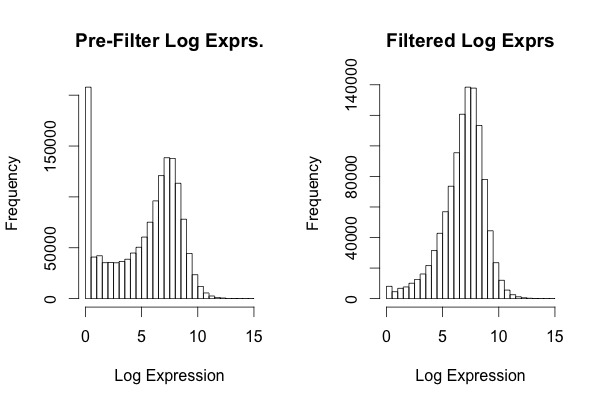
\includegraphics[width=\textwidth]{../../fig/filter_histograms.png}
\caption{\textbf{Histogram.} The histogram on the left shows the log of the abundance estimates looking
  approximately normal, but with a large spike at 0.  On the right, we see the
  histogram of the log of the abundance estimates after filtering and note that the spike at 0 is
  reduced.}
   \label{fig:histogram}
\end{figure}

We next investigated the need for normalization.  In Figure~\ref{fig:boxplot}
on page~\pageref{fig:boxplot}, we have displayed boxplots of the filtered
log-transformed abundance estimates for all the subjects in our dataset.  The
boxplots reveal no visually obvious difference between KIRC and KIRP cells.
But they do reveal variability that suggests the need for normalization.
For the purposes of this project, we decided to use upper quartile normalization.
In Figure~\ref{fig:boxplotpost} on page~\pageref{fig:boxplotpost}, we've displayed
the normalized log-transformed abundance estimates for the validation set where
the normalization was based on the upper-quartile normalization of the training
set.  In Figure~\ref{fig:histogrampost} on page~\pageref{fig:histogrampost},
we display the post-normalization histogram for the training set.

\begin{figure}[H]
  \centering
    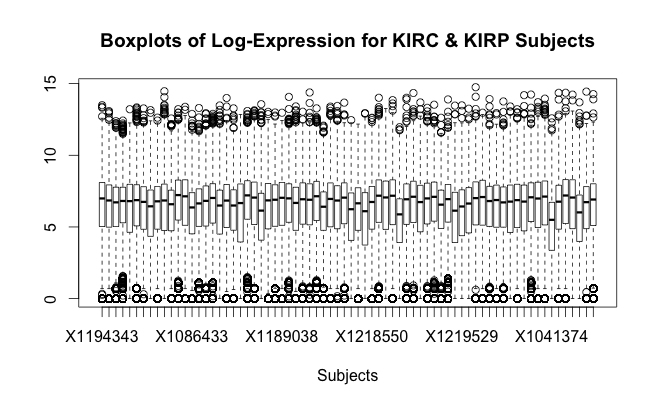
\includegraphics[width=\textwidth]{../../fig/postfilter_boxplot.png}
\caption{\textbf{Boxplot.} This figure shows box plots of the distributions of
  log of the abundance estimates for all 72 subjects in our dataset (after filtering). Red 	box
  plots correspond to subjects in the KIRC group, while blue box plots correspond
  to those in the KIRP group. No notable differences between KIRC and KIRP
  subjects are shown in these box plots.}
   \label{fig:boxplot}
\end{figure}


\begin{figure}[H]
  \centering
    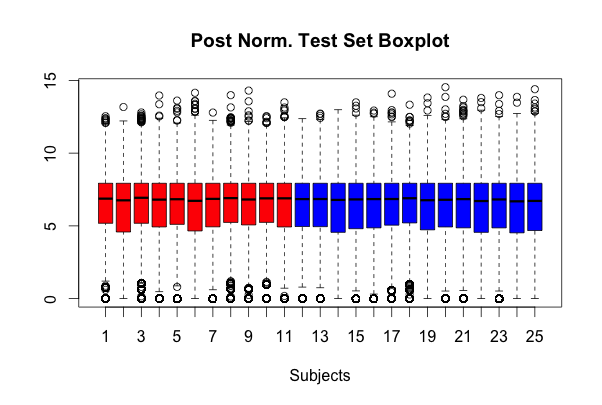
\includegraphics[width=.8\textwidth]{../../fig/postnorm_test_boxplot.png}
\caption{\textbf{Test Set Boxplots after normalization.} After applying the training
  set normalization onto the test set, here is what the distributions of the
  log of the abundance estimates for the test subjects look like. Notice, all of the upper quantiles
  are aligned as expected with upper quantile normalization.}
   \label{fig:boxplotpost}
\end{figure}


\begin{figure}[H]
  \centering
    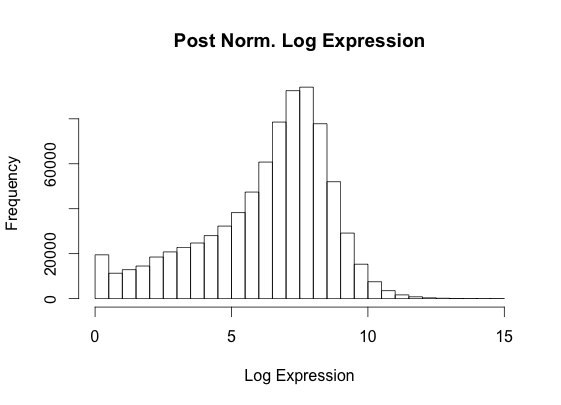
\includegraphics[width=.8\textwidth]{../../fig/postnorm_histogram.png}
\caption{\textbf{Histogram after normalization.} This histogram shows the distribution
  of the log of the abundance estimates in the training set, after applying upper quantile
  normalization. It looks very similar to the original histogram of the
  log of the abundance estimates after filtering out low abundance genes.}
   \label{fig:histogrampost}
\end{figure}

After normalization and low abundance estimates filtering, we attempt to select the
best genes to feed into the Support Vector Machines and Linear Discriminant
Analysis classifiers.  We first produced a list of the genes with the largest
variances across KIRC and KIRP subjects.
%The top $N_{best}$ genes are presented in Table Y.
Additionally, we produced a list of p-values for
differential expression of genes in the two cancer types.

%Table X summarizes
%the genes with the smallest p-values. Fig. Y shows a histogram of the p-values
%with lines showing typical significance levels. 

In Figure~\ref{fig:pca} on page~\pageref{fig:pca}, we plot the scores
corresponding to the first two principal components and colored the points
according the cancer cell type.  Evidently, the two cancer types separate
nicely along the first principal component. This is not too surprising since we ran the PCA analysis on the genes that show large differences in expression according to our t-test feature selection method.   The PCA analysis shows that the assumption that our data is linearly separable is reasonable. Thus it is reasonable to use LDA and SVM. 

\begin{figure}[H]
  \centering
    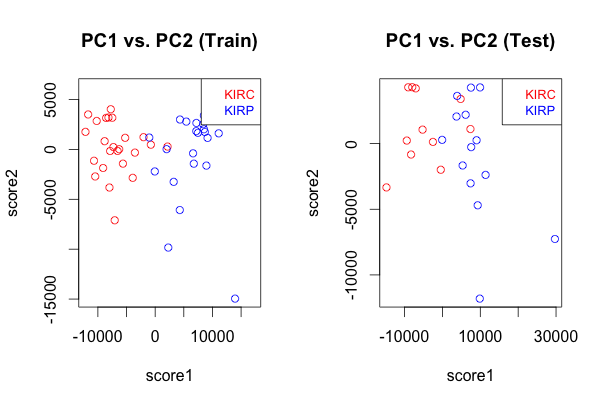
\includegraphics[width=.8\textwidth]{../../fig/pcplot.png}
\caption{\textbf{PCA Plot.} Principal Component 1 is on the x-axis and Principal
  Component 2 is on the y-axis for both scatterplots.  PCA is performed on the
  training set (with the 40 p-value selected genes) and applied to the test set.
  In both plots, we see a clear divide between 	KIRC and KIRP subjects along
  the first principal component.}
   \label{fig:pca}
\end{figure}

For each distinct combination of feature selection procedure and the LDA and
SVM classifiers, we built classification models on the training set.

Using the LDA classifier learned from the training set, we get the following
confusion matrix when applied to the validation set:

%\vspace*{\fill}
\begin{quote}{  \ttfamily \raggedright \noindent
\centering
~~~Variance~~~~~~~~~~~~~~~~~Tscore\\
~\\
~~~~~~true~~~~~~~~~~~~~~~~~~~~true\\
pred~~~KIRC~KIRP~~~~~~~~pred~~~KIRC~KIRP\\
~~KIRC~~~~7~~~~5~~~~~~~~~~KIRC~~~~8~~~~3\\
~~KIRP~~~~4~~~~9~~~~~~~~~~KIRP~~~~3~~~11\\
}
\end{quote}
%\vspace*{\fill}

LDA performs better when feature selection is based on the test score ranking.

Using the SVM classifier learned from the training set, we get the following
confusion matrix when applied to the validation set:

%\vspace*{\fill} 
\begin{quote}{ \ttfamily \raggedright \noindent
\centering
~~~Variance~~~~~~~~~~~~~~~~~Tscore\\
~\\
~~~~~~true~~~~~~~~~~~~~~~~~~~~true\\
pred~~~KIRC~KIRP~~~~~~~~pred~~~KIRC~KIRP\\
~~KIRC~~~~7~~~~0~~~~~~~~~~KIRC~~~~9~~~~0\\
~~KIRP~~~~4~~~14~~~~~~~~~~KIRP~~~~2~~~14\\
}
\end{quote}
%\vspace*{\fill}

SVM performs better than LDA and performs better when feature selection is
based on the test score ranking, rather than variance ranking.

Using the RF classifier learned from the training set, we get the following
confusion matrix when applied to the validation set:

%\vspace*{\fill}
\begin{quote}{ \ttfamily \raggedright \noindent
\centering
~~~~~~true\\
pred~~~KIRC~KIRP\\
~~KIRC~~~~8~~~~0\\
~~KIRP~~~~3~~~14\\
}
\end{quote}
%\vspace*{\fill}

RF performs better than LDA and almost identical to SVM.

\begin{figure}[H]
  \centering
    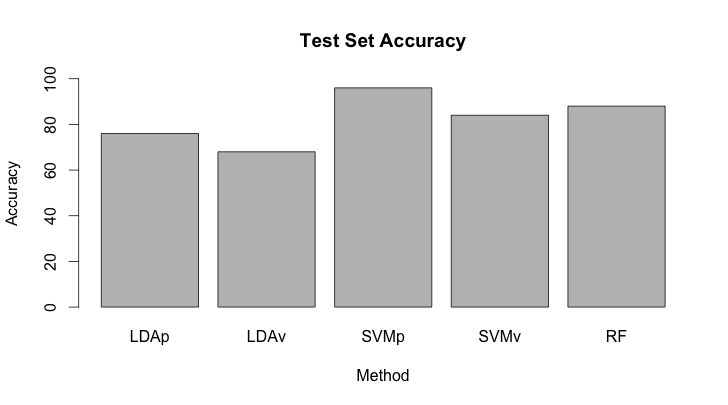
\includegraphics[width=.8\textwidth]{../../fig/testset_acc.png}
\caption{\textbf{Performance.}This bar plot compares the percentages of correctly
  classified subjects, that our classification methods achieve. We see that
  Support Vector Machines (with the p-value subset of genes) performs the best
  with 96\% accuracy. Linear Discriminant Analysis (on the variance subset of
  genes) performs the worst at 68\%.}
   \label{fig:performance}
\end{figure}

The proportion of correctly classified subjects for each of the methods using
the smallest p-value subset of genes is as follows:

\begin{enumerate}
\item Support Vector Machine - $Accuracy = 92\%$
\item Linear Discriminant Analysis - $Accuracy = 76\%$
\end{enumerate}

The proportion of correctly classified subjects for each of the methods using
the largest variance subset of genes is as follows:

\begin{enumerate}
\item Support Vector Machine - $Accuracy = 84\% $
\item Linear Discriminant Analysis - $Accuracy =64\% $
\end{enumerate}

Random Forest is not built on a subset of the genes in our dataset, but rather
all of the genes. It is allowed to determine the best subset of genes for
classification of cell type. The proportion of correctly classified validation
subjects using Random Forest is $88\%$.

The classifier that best predicts cancer cell types in the validation set is
Support Vector Machine, correctly predicting for $24$ out of $25$ subjects.
In Figure~\ref{fig:performance} on page~\pageref{fig:performance}, we
summarize the performance of each classifier (and feature selection
method) in terms of its accuracy in prediction on the validation set.

\subsection*{Reproducibility}

All code, figures, and text for this project are available on Github.\footnote{\url{https://github.com/jarrodmillman/ph240f}}


\section{Discussion}

Our results are fundamentally limited due to the data. As this data was not
designed for this type of experiment, necessary controls are not in place. For
instance, the differences between gene expression may be due to technical
effects. We do not have batch information for the subjects, so we cannot try to
correct for possible batch effects. Figure~\ref{fig:mdplot} on
page~\pageref{fig:mdplot} shows Mean-Difference Plots of subjects within the
same cancer cell type and of subjects with differing cell types.  This is
problematic because differences in expression between groups may be due to
technical effects as opposed to biological effects of interest.  In our feature
selection, we might be unknowingly, choosing genes on which to build the
classifiers that reflect the technical effects, and not those that reflect
biological differences between subjects with KIRC and KIRP.

\begin{figure}[H]
  \centering
    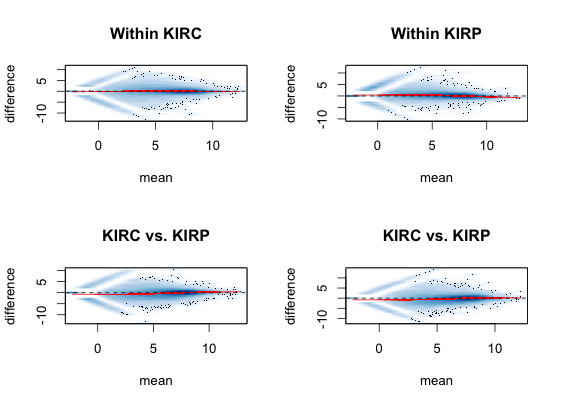
\includegraphics[width=\textwidth]{../../fig/mdplots_postnorm.png}
\caption{\textbf{MD plots.} Above are Mean Difference Plots after normalization, to
  compare the magnitude of the differences in expression between subjects with
  the same type of cancer cell and between subjects with different types.  Note
  that, for same cell type subjects, the differences displayed in the plots look
  very similar to those seen in the plots for different cell type subjects. This
  is possibly due to some technical effects (such as Batch
  effect) that we were unable to investigate.}
   \label{fig:mdplot}
\end{figure}


From these plots, we see that the magnitude of technical effects within a cell
type is similar to the magnitude of the biological effects between cell types
which interest us. Also, the RNA-Seq experiments were carried out a few months
apart. It is not clear what efforts were made to standardize the procedure of
processing the cancer samples. In the future, it would be important to have a
negative control where two samples that are supposed to be the same are
processed at during the two times that the cancer cells were processed. 

Nonetheless, all of our classification methods appear to satisfactorily predict
cancer cell type in new patients, given their expression in some selected
genes. The classifiers using the subset of genes determined by ranked p-values
performed slightly better than the classifiers built with the subset of genes
with the largest variances.

In the future, we have a number of things that we can do to extend and improve our analysis. The first thing that would should do is get error bars on our accuracy estimates for each method that we used. The simplest way to go about this would be to do a $k$-fold cross validation scheme. Next, it would be important to collaborate with the biologists who generated this data to better understand the biological significance of the genes that we identified using our feature selection methods. Furthermore, there may be biological nuissance effects such as gender or age that impact our results. 

Additionally, it would be useful to incorporate healthy kidney cell RNA-Seq data into our data set. We could, for instance, run a classifier that has three classifications where the third classification is not having cancer. Relatedly, it would be helpful if, in our current scheme, we had confidence estimates in our classifications. For instance, in an actual biological application, it would be important to have a scheme for saying that we aren't confident enough to give a classification. 

Finally, we could do more to assess the robustness of our methods to changing various parameters in our analysis. For instance, we chose $40$ genes, but we can vary that number and see how the accuracy of our classifiers change. Also we chose upper quantile normalization for our analysis, but other normalization schemes could be assessed as well. 



\section*{Acknowledgments}

We would like to thank Davide Risso for pointing us to the Cancer Genome Atlas
as well as providing feedback on our proposal. Sandrine Dudoit and Haiyan Huang
offered us important feedback on our initial proposals as well as on our
intermediate results. 

\bibliographystyle{imsart-number} %bibliographystyle{imsart-nameyear}
\bibliography{kidney}

\end{document}
